\section{Network Flow}
A flow network is a grap G=(V,E) with source $s \in V$ and $t \in V$, with $\forall e \in E, \; c(e) \geq 0$.An $s \rightarrow t$ cut is a partition (A, B) of the vertices with $s \in A$ and $ t \in B$, while the capacity is the sum of all the capacities of all the edges from A to B: cap(A,B) = $ \sum_{e \; out \; of \; A}^{} c_{e}$

\begin{figure}[H]
    \centering
    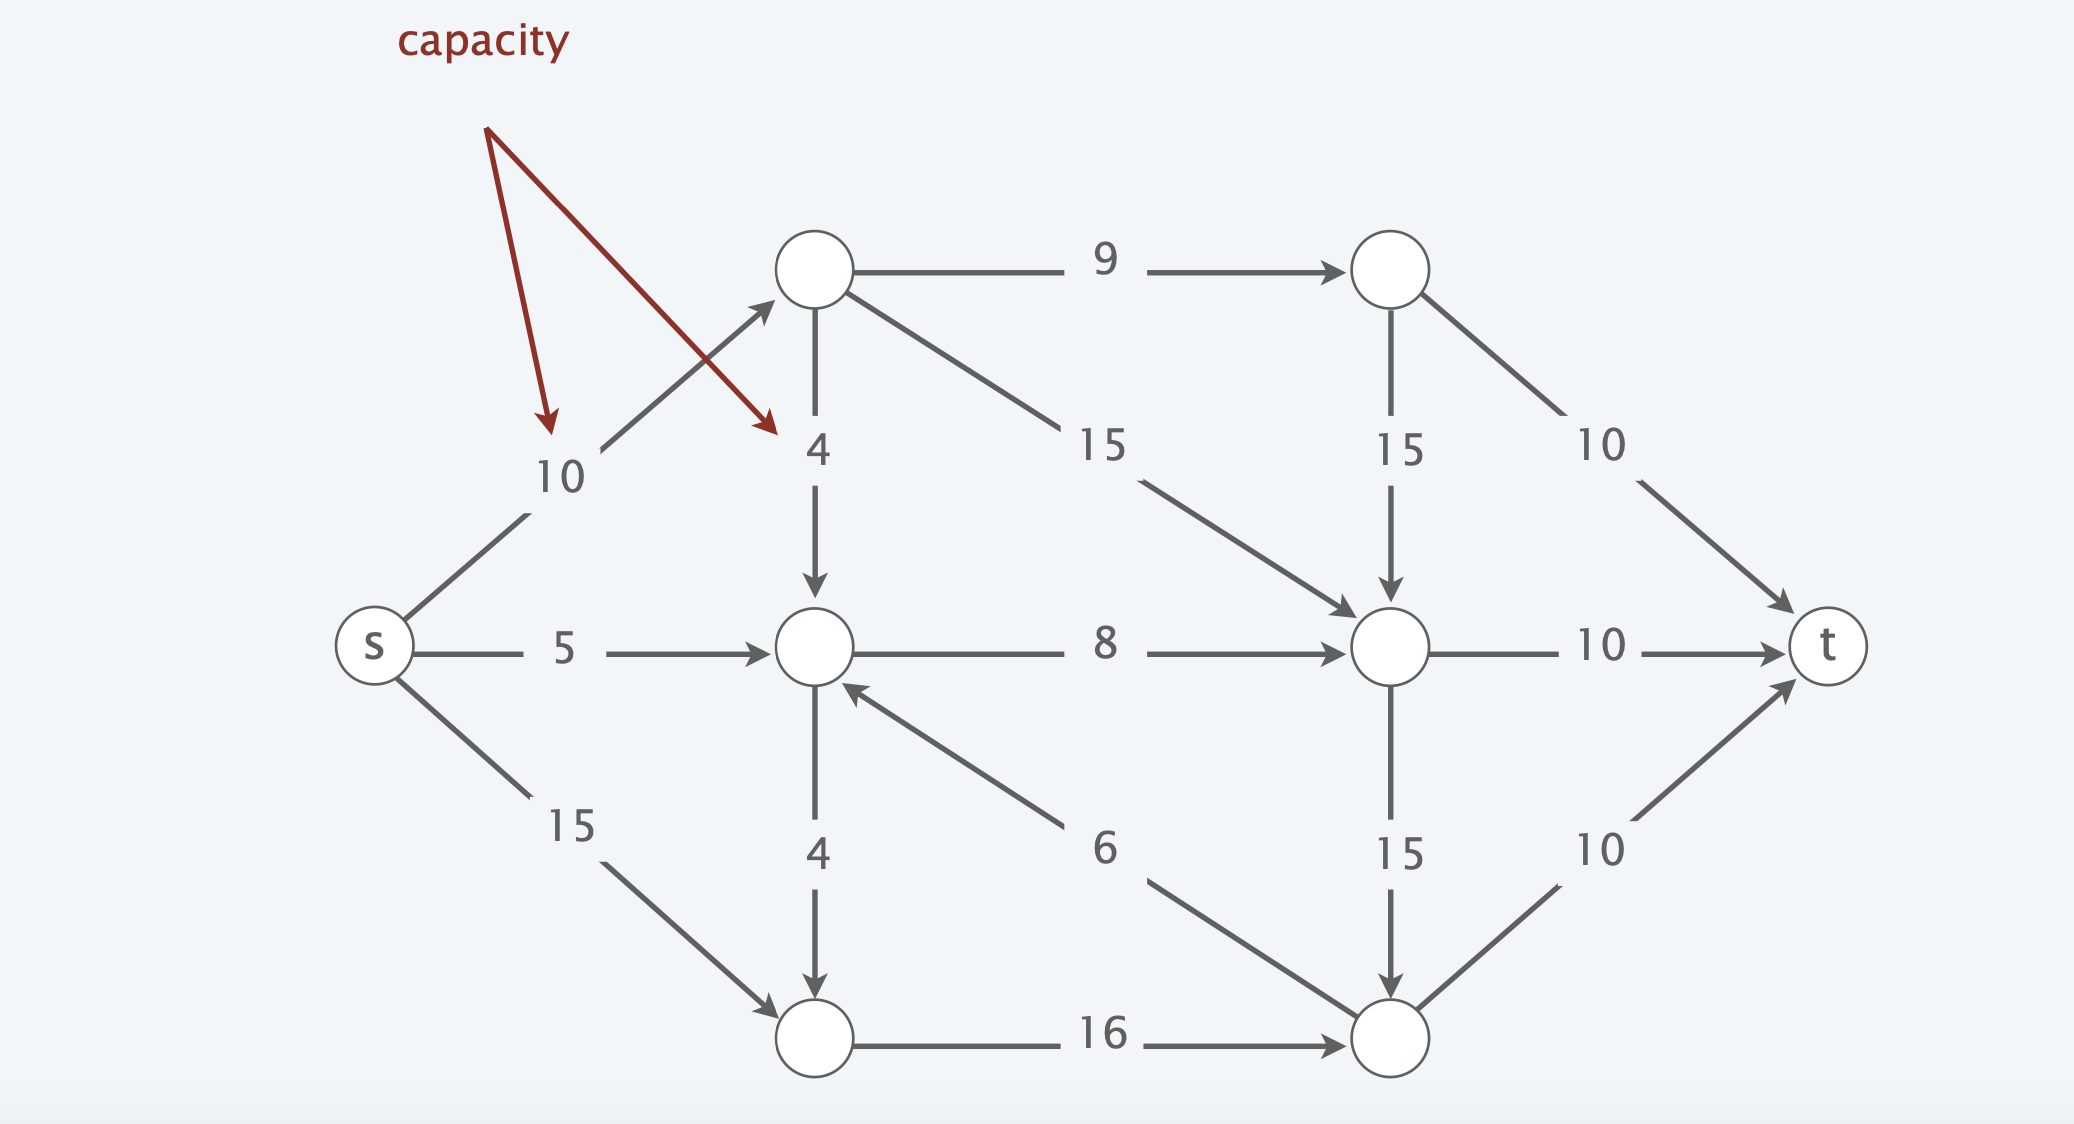
\includegraphics[width=0.5\textwidth ]{network1}
    \caption{An instance of network flow.}
\end{figure}

\subsection{The Maximum Flow Problem}
An $s \rightarrow t$ is a function f that satisfies:

\[ \forall e \in E: \; 0 \leq f(e) \leq c(e) \; (capacity)\]

\[ \forall v \in V - \{s, t\}: \sum_{e \; out \; of \; v}^{} f(e) = \sum_{e \; into \; v}^{} f(e) \; (flow \; conservation)\]

The maximum flow problem, aim at maximizing the flow function, while respecting the constraint above.

\subsection{The maximum flow/ minimum cut relationship}

\begin{itemize}

    \item{Residual Graph}

          \begin{figure}[H]
              \centering
              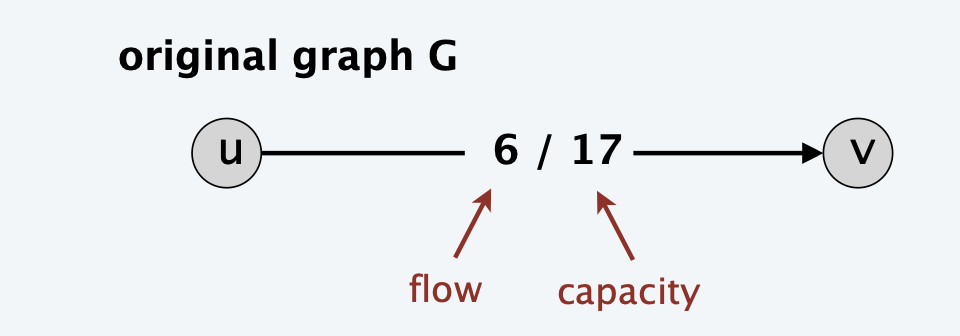
\includegraphics[width=0.3\textwidth ]{residual2}
              \caption{The orignal flow}
          \end{figure}

          \begin{figure}[H]
              \centering
              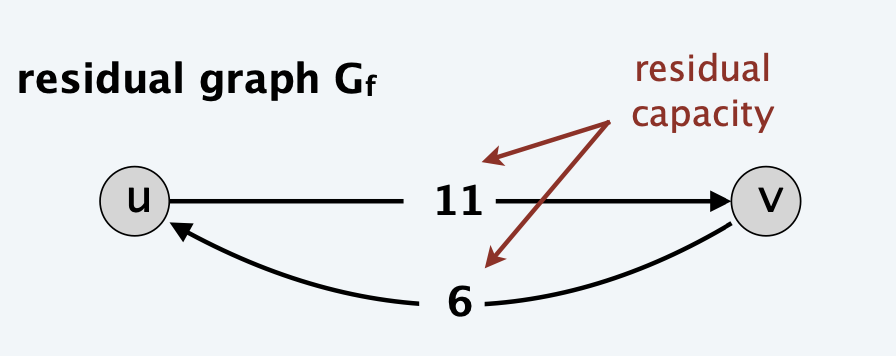
\includegraphics[width=0.3\textwidth ]{residual1}
              \caption{The residual edge.}
          \end{figure}

          The residual graph G is simply the graph resulting upon applying the residual transformation $\forall e \in E$

    \item{Augmenting Path}\\
          An augmenting path is a simple $s \leftarrow t$ path P in the residual graph $G_{f}$, The bottleneck capacity of an augmenting P is the minimum residual capacity of any edge in P.

    \item {Flow value Lemma}\\
          Let f be any flow and let (A, B) be any cut. Then, the net flow across (A, B) equals the value of f:

          \[ \sum_{e \; out \; of \; A}^{} f(e) = \sum_{e \; into \; A}^{} f(e) = v(f)\]

          proof:

          \[v(f) = \sum_{e \; outof  \; s}^{} f(e) =  \sum_{v \in A}^{} ( \sum_{e \; out of  \; v}^{} f(e) - \sum_{e \; into  \; v}^{} f(e)) =  ( \sum_{e \; out of  \; A}^{} f(e) - \sum_{e \; into  \; A}^{} f(e))\]

    \item {Weak Duality}\\
          Let f be any flow and (A, B) be any cut. Then, v( f ) $\leq$ cap(A, B).

          proof:

          \[v(f) =  \sum_{e \; out of  \; A}^{} f(e) - \sum_{e \; into  \; A}^{} f(e) \leq  \sum_{e \; out of  \; A}^{} f(e) \leq \sum_{e \; out of  \; A}^{} c(e) = cap(A,B)\]

    \item {Integrality Theorem}\\
          If c(e) $\forall e \in E$ are integers, then there exists a max flow f for which every flow value f(e) is an integer.

\end{itemize}

\begin{claim}
    The value of the maximum flow equals to the minimum cut, furthermore, when the flow is maximized there are no augmenting path left.
\end{claim}\\

\begin{proof}
    If there exists a cut (A, B) such that cap(A, B) = val(f),there is no augmenting path with respect to f, so f is a max-flow.
\end{proof}

\subsection{Ford-Fulkerson Algorithm}
It's a simple greedy approach algorithm: basically we start with a f(e) = 0 $\forall e \in E$, then we will find all the augmenting path in G(V,E) until there are no more left, the result is both a maximum flow and an min-cut.\\

\begin{algorithm}[H]
    \SetAlgoLined
    \small
    \KwIn{$G$ directed graph \; $s$ source node of the flow, $t$ sink of the flow.}
    \KwOut{$S$ containing all the paths that maxes the maximum flow. $\leftarrow$ t}

    \BlankLine


    \BlankLine

    \caption{FordFulkerson(G,s,t):}
\end{algorithm}

\begin{claim}
    The Ford-Fulkerson complexity is $\mathcal{O}(|E|f^{*})$
\end{claim}\\

\begin{proof}
    the algorithm terminates only when there are no more augmenting paths on G and by definition there is no more flow in the residual net $f^{*}$. Since the algorithm needs to check all the augmenting paths until there are no more left, the execution is closely releated on how many augmenting paths are in G.
\end{proof}

\subsection{Matching and Bipartite Matching}

\emph{Formal definition}: Given an undirected graph G = (V, E) a subset of edges $M \subseteq E$ is a matching if each node appears in at most one edge in M, the maximum matching is a max cardinality matching.

\begin{figure}[H]
    \centering
    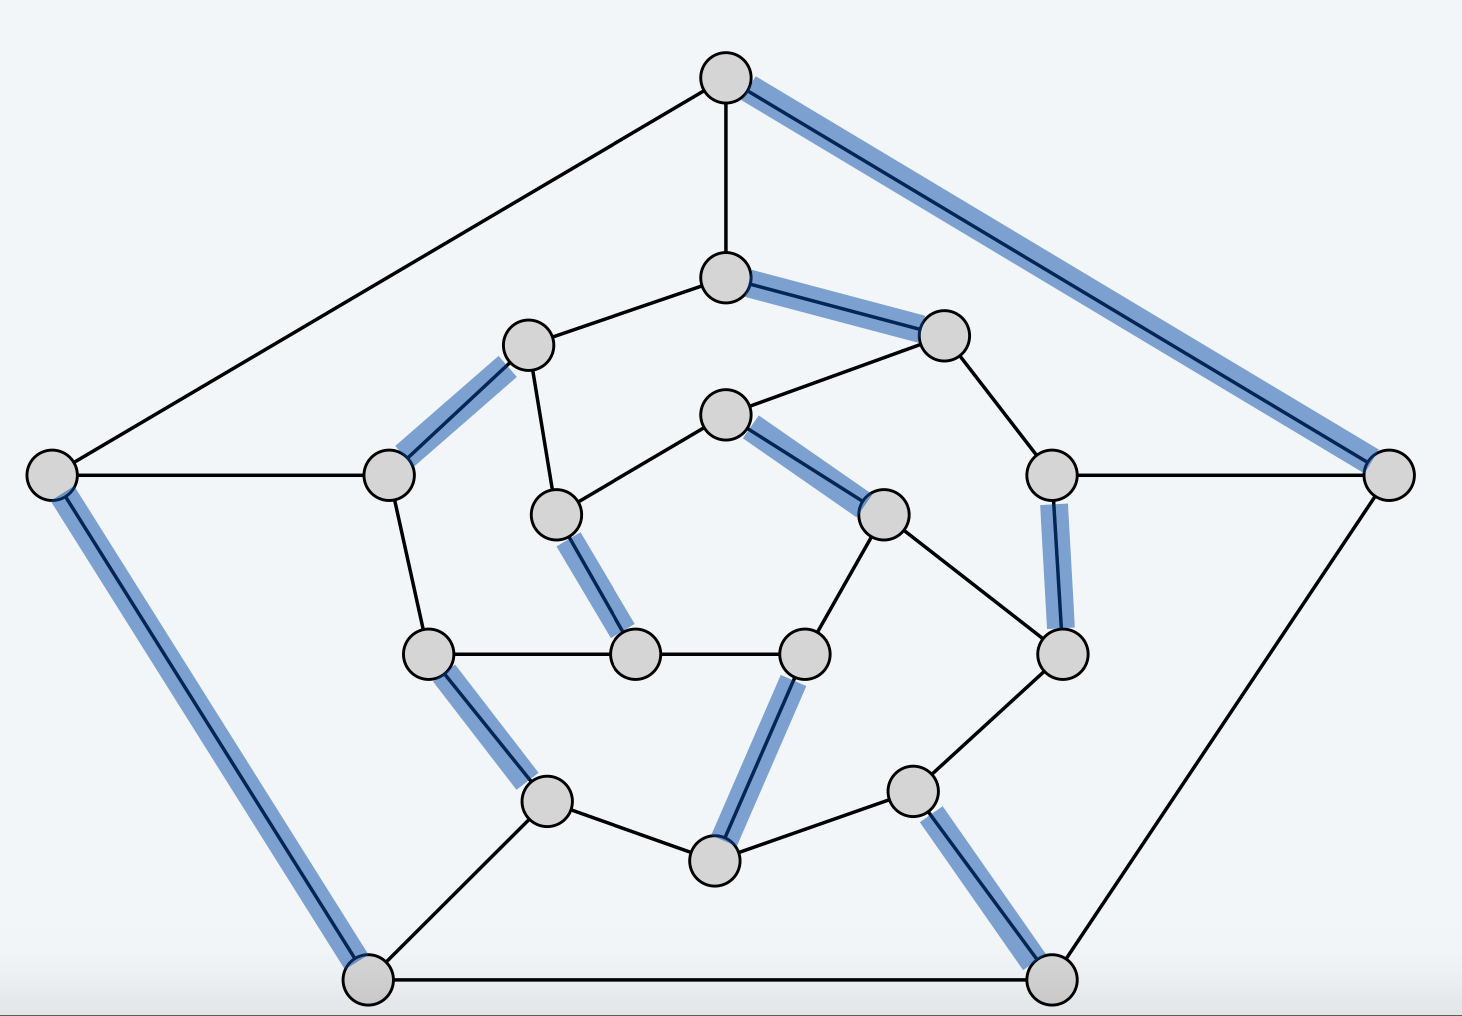
\includegraphics[width=0.5\textwidth ]{matching}
    \caption{The maximum matching in a Graph G}
\end{figure}

\emph{Formal definition}: A graph G is bipartite if the nodes can be partitioned into two subsets L (Left) and R (Right) such that every edge connects a node in L to one in R, a bipartite matching G = (L $\cup$ R, E), find a max cardinality matching.

\begin{figure}[H]
    \centering
    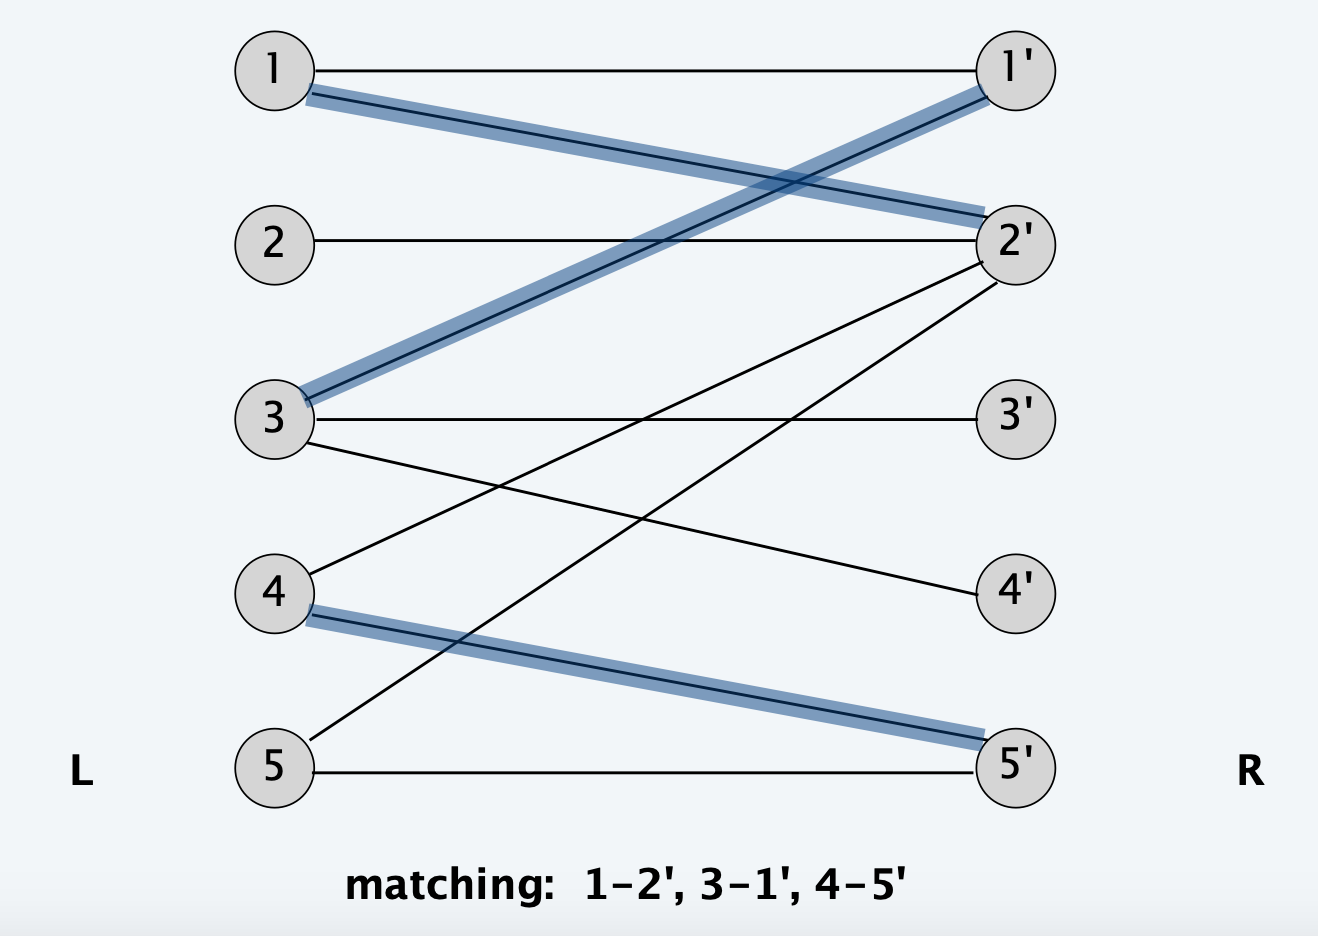
\includegraphics[width=0.5\textwidth ]{bmatching}
    \caption{The maximum bipartite matching in a Graph G}
\end{figure}


\emph{Hall Theorem}: Let S be a subset of nodes, and let N(S) be the set of nodes adjacent to nodes in S, Let $G = (L \cup R, E)$ be a bipartite graph with $|L| = |R|$. G has a perfect matching iff $|N(S)| \geq |S|$ for all subsets $S \subseteq L$.\\

\clearpage

\emph{Proof}: Suppose G does not have a perfect matching: formulate a max flow problem and let (A, B) be min cut in G', by max-flow min-cut theorem: $cap(A, B) < | L |$.\\
Define LA=$L\cap A, LB=L \cap B, RA=R \cap A$, so the cap(A, B) = $| LB | + | RA |$. Since min cut can't use $\infty$ edges: $N(LA) \subseteq RA \; with \; |N(LA)| \leq |RA|$ = $cap(A,B) – |LB| < |L| – |LB| = |LA|$ so S=LA.

\begin{figure}[H]
    \centering
    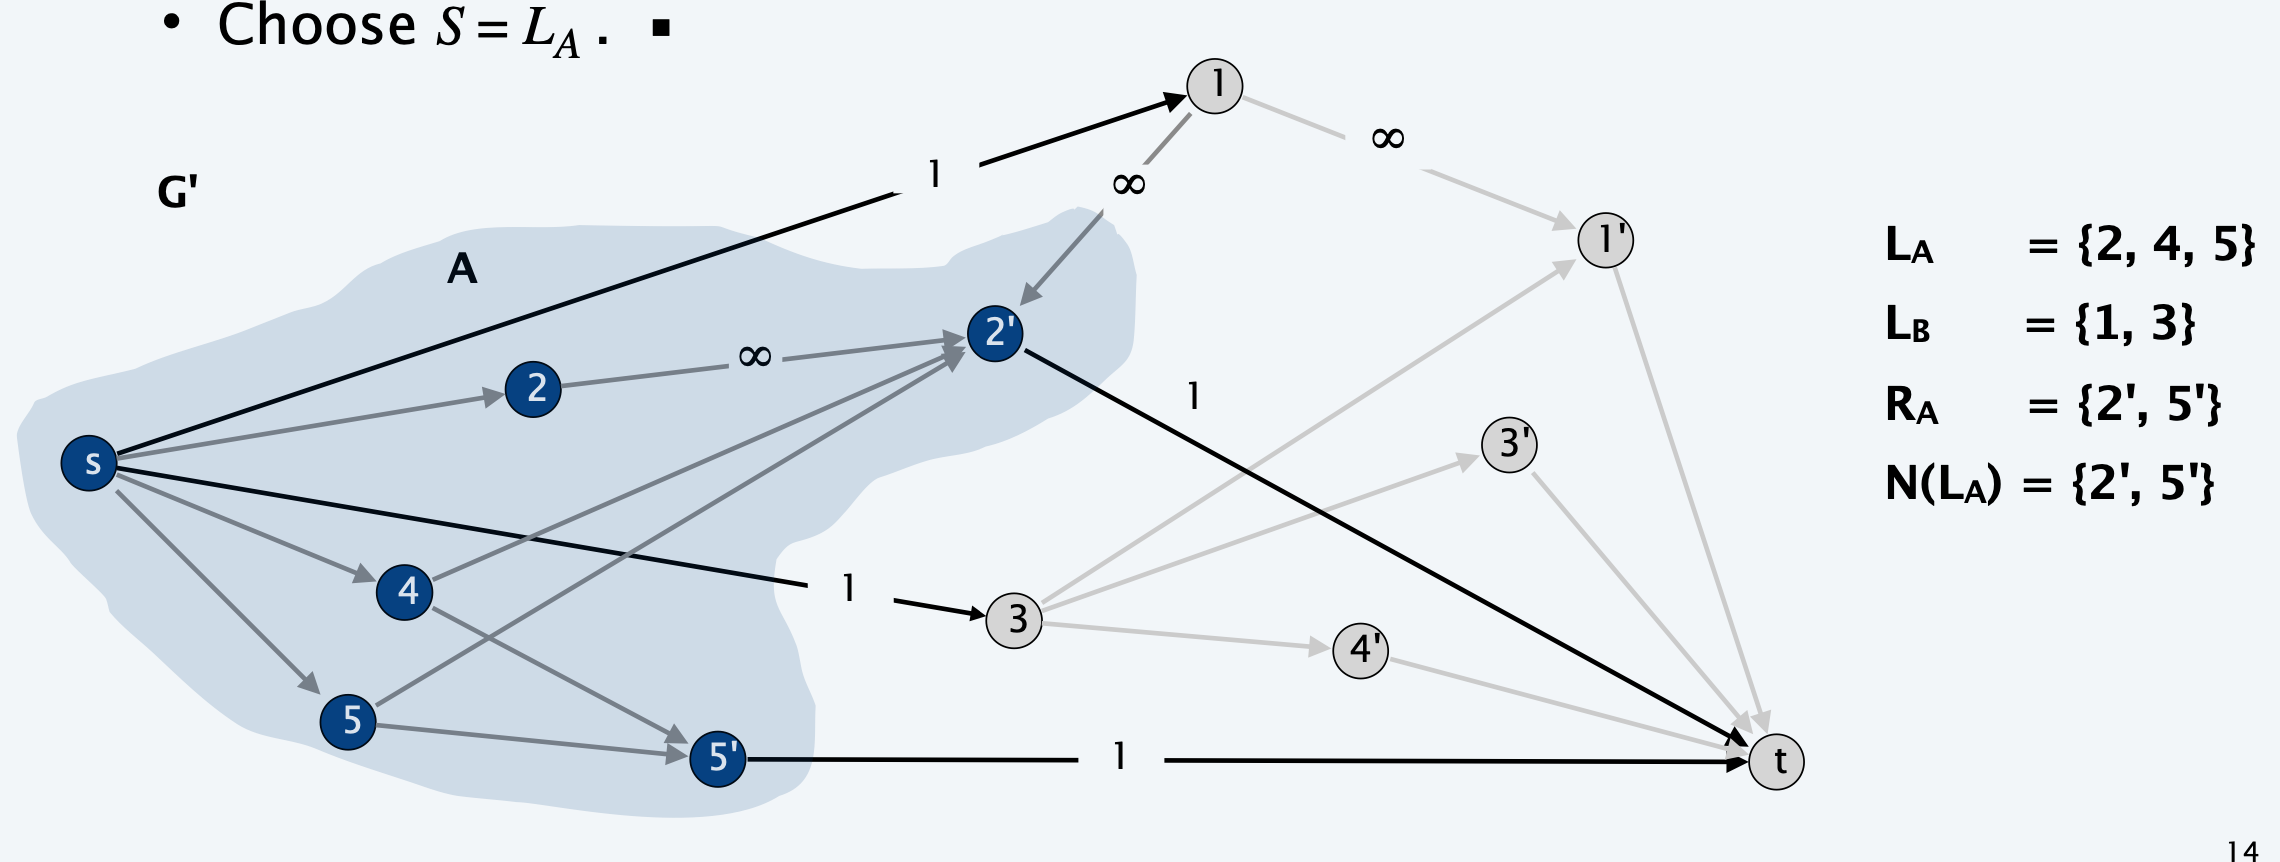
\includegraphics[width=0.8\textwidth ]{hall}
    \caption{}
\end{figure}


\begin{claim}
    The max cardinality of a matching in G = value of max flow in G'.
\end{claim}\\

\begin{proof}
    First we need to build $G_{'} = (L \cup R \cup \{s, t\}, E^{'} )$ , direct all edges from L to R and give them unit capacity, then connect s to all $e \in L$ and t to all $e \in R$ with edges with infinite capacity, using the integrality theorem we know that the flow can assume only value 0-1. Finally consider the set of edges from L to R with f (e) = 1, each node in L and R participates in at most one edge in M, with with f (e) = 1 so $| M | = k$: considering the  cut ($L \cup s, R \cup t$).
\end{proof}

\subsection{Edge Disjointed Paths}
\emph{Definition}:Two paths are edge-disjoint if they have no edge in common.\\\\
\emph{Edge Disjointed Problem}: Given a digraph G = (V, E) and two nodes s and t, find the max number of edge-disjoint $s \Rightarrow t$ paths.


\begin{figure}[H]
    \centering
    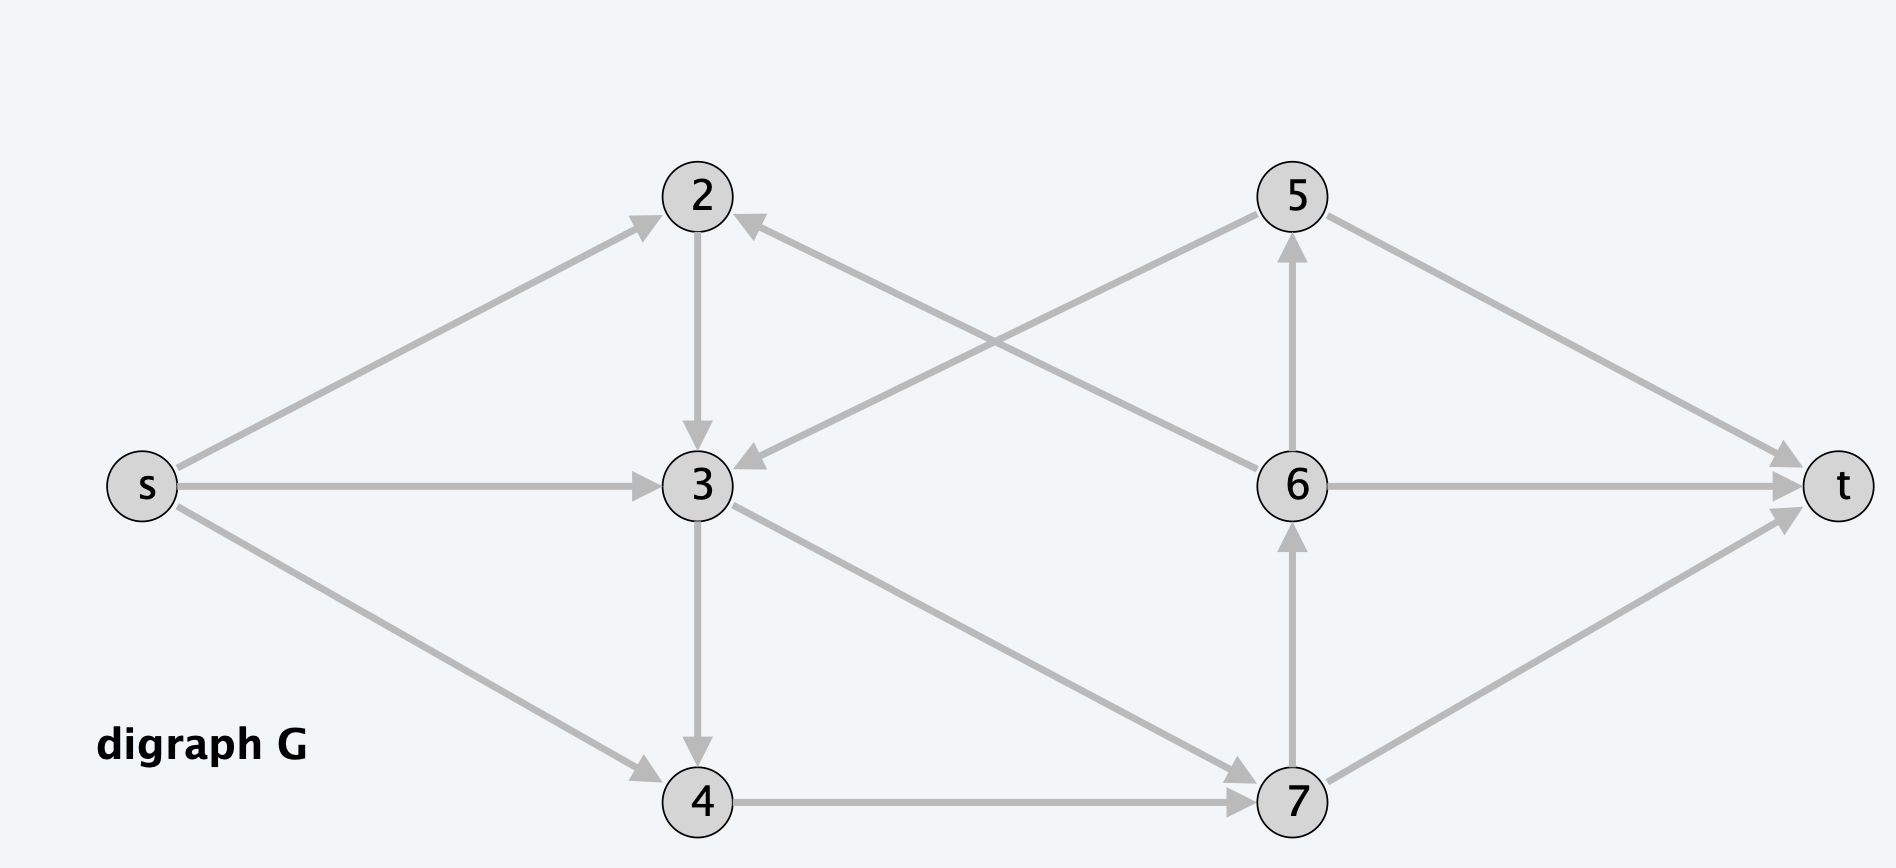
\includegraphics[width=0.6\textwidth ]{disjointed}
    \caption{Instance of the Disjointed Path problem}
\end{figure}

\begin{claim}
    Given a digraph G=(V,E) with $c(e) = 1,\; \forall e \in E$ the max number edge-disjoint $s \Rightarrow t $ paths equals value of max flow.
\end{claim}\\

\begin{proof}
    Suppose max flow value is k: Integrality theorem $ \Rightarrow $  there exists 0-1 flow f of value k. Now Consider edge (s, u) with f(s, u) = 1.\\
    By conservation, there exists an edge (u, v) with f(u, v) = 1 continue until reach t, always choosing a new edge, the solution produces k (not necessarily simple) edge-disjoint paths.
\end{proof}\\

\begin{figure}[H]
    \centering
    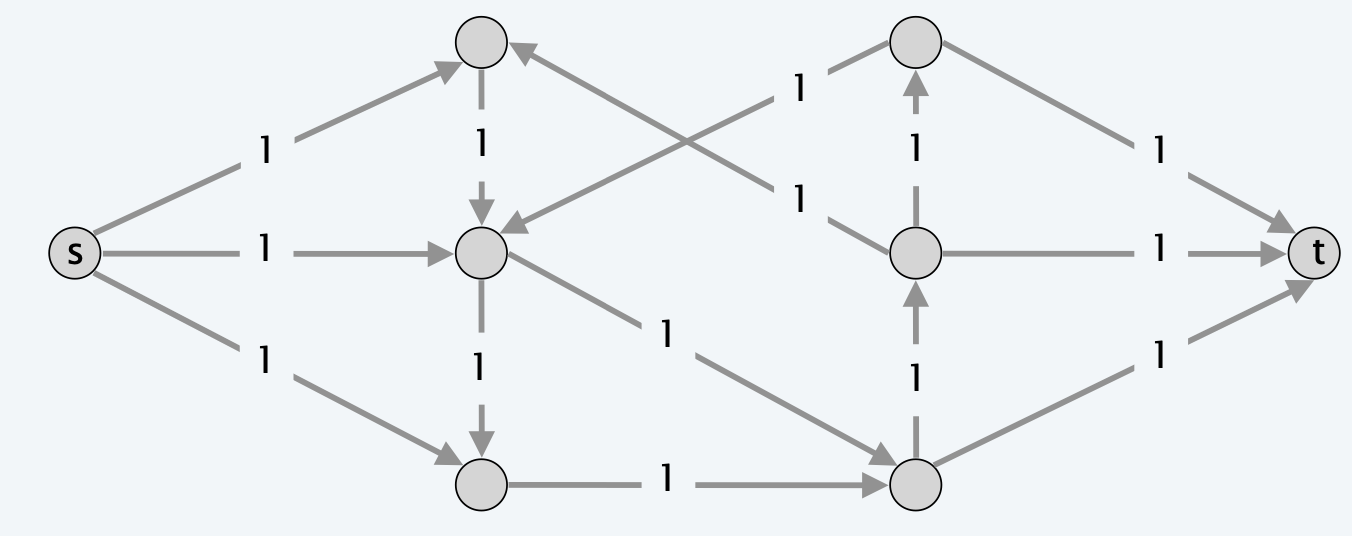
\includegraphics[width=0.6\textwidth ]{maxFlowDisjointed}
    \caption{Instance of the Disjointed Path problem}
\end{figure}

\begin{claim}
    \emph{Manger's Theorem}: The max number of edge-disjoint $s \Rightarrow t$ paths is equal to the min number of edges whose removal disconnects t from s.
\end{claim}\\

\begin{proof}
    Suppose max number of edge-disjoint paths is k: then value of max flow = k, using the max-flow min-cut theorem $  \Rightarrow $ there exists a cut (A, B) of capacity k. Let F be set of edges going from A to B.
    $|F| = k$ and disconnects t from s.
\end{proof}\\

The Manger's theorem can even be applied to undirected graphs: (it's always possible to transform an undirected graph to directed by simply replacing every edge (u,v) with 2 direct edges (u,v) and (v,u)), then the formulation and proof is the same as above.

\subsection{Circulation With demands}
Given a digraph G = (V, E) with nonnegative edge capacities c(e) and node supply and demands d(v), a circulation is a function that satisfies:

\[ \forall e \in E: \; 0 \leq f(e) \leq c(e) \; (capacity)\]

\[ \forall v \in V: \sum_{e \; out \; of \; v}^{} f(e) = \sum_{e \; into \; v}^{} f(e) = d(v) \; (flow \; conservation)\]

\begin{figure}[H]
    \centering
    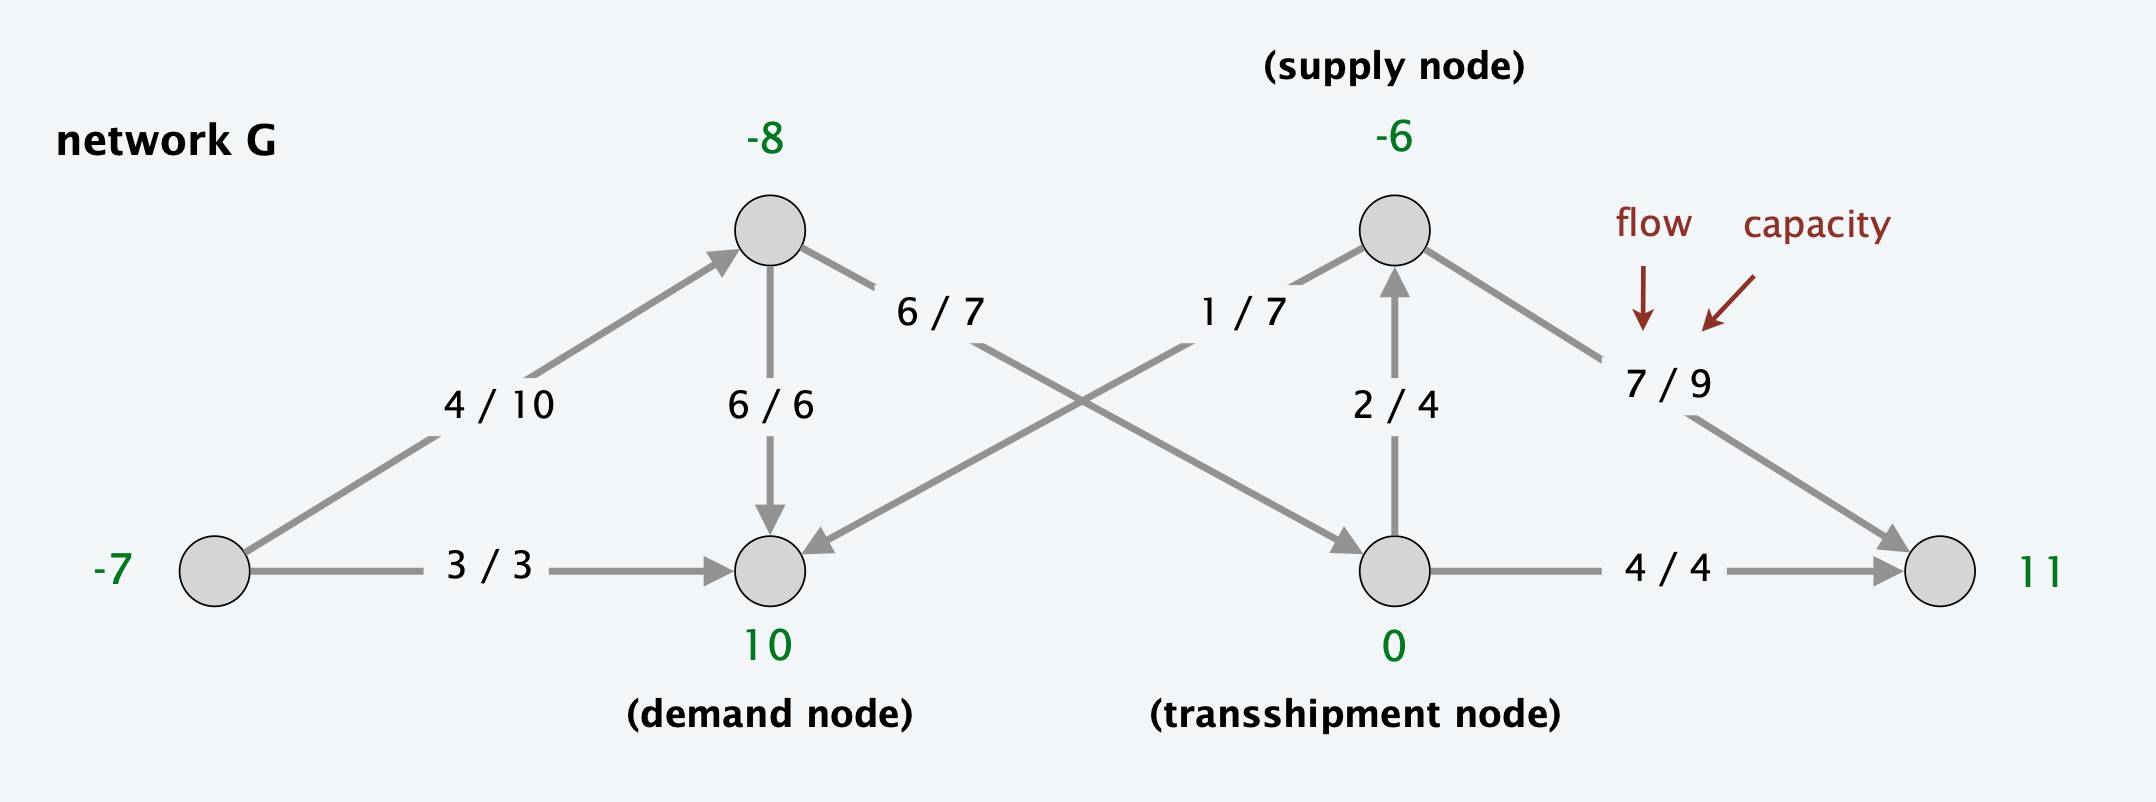
\includegraphics[width=0.6\textwidth ]{circulation}
    \caption{Instance of the Circulation problem}
\end{figure}

In order to transform the circulation into a flow problem we need to connect the source s to each node with $d(v) < 0$ and t with each node with $d(v) > 0$.\\
The original Graph G has a circulation if G' has a max flow of value:
\[ \sum _{v \: in \; d(v) > 0 } d(v) = \sum _{v \; in \; d(v) < 0} - d(v)\]

\begin{figure}[H]
    \centering
    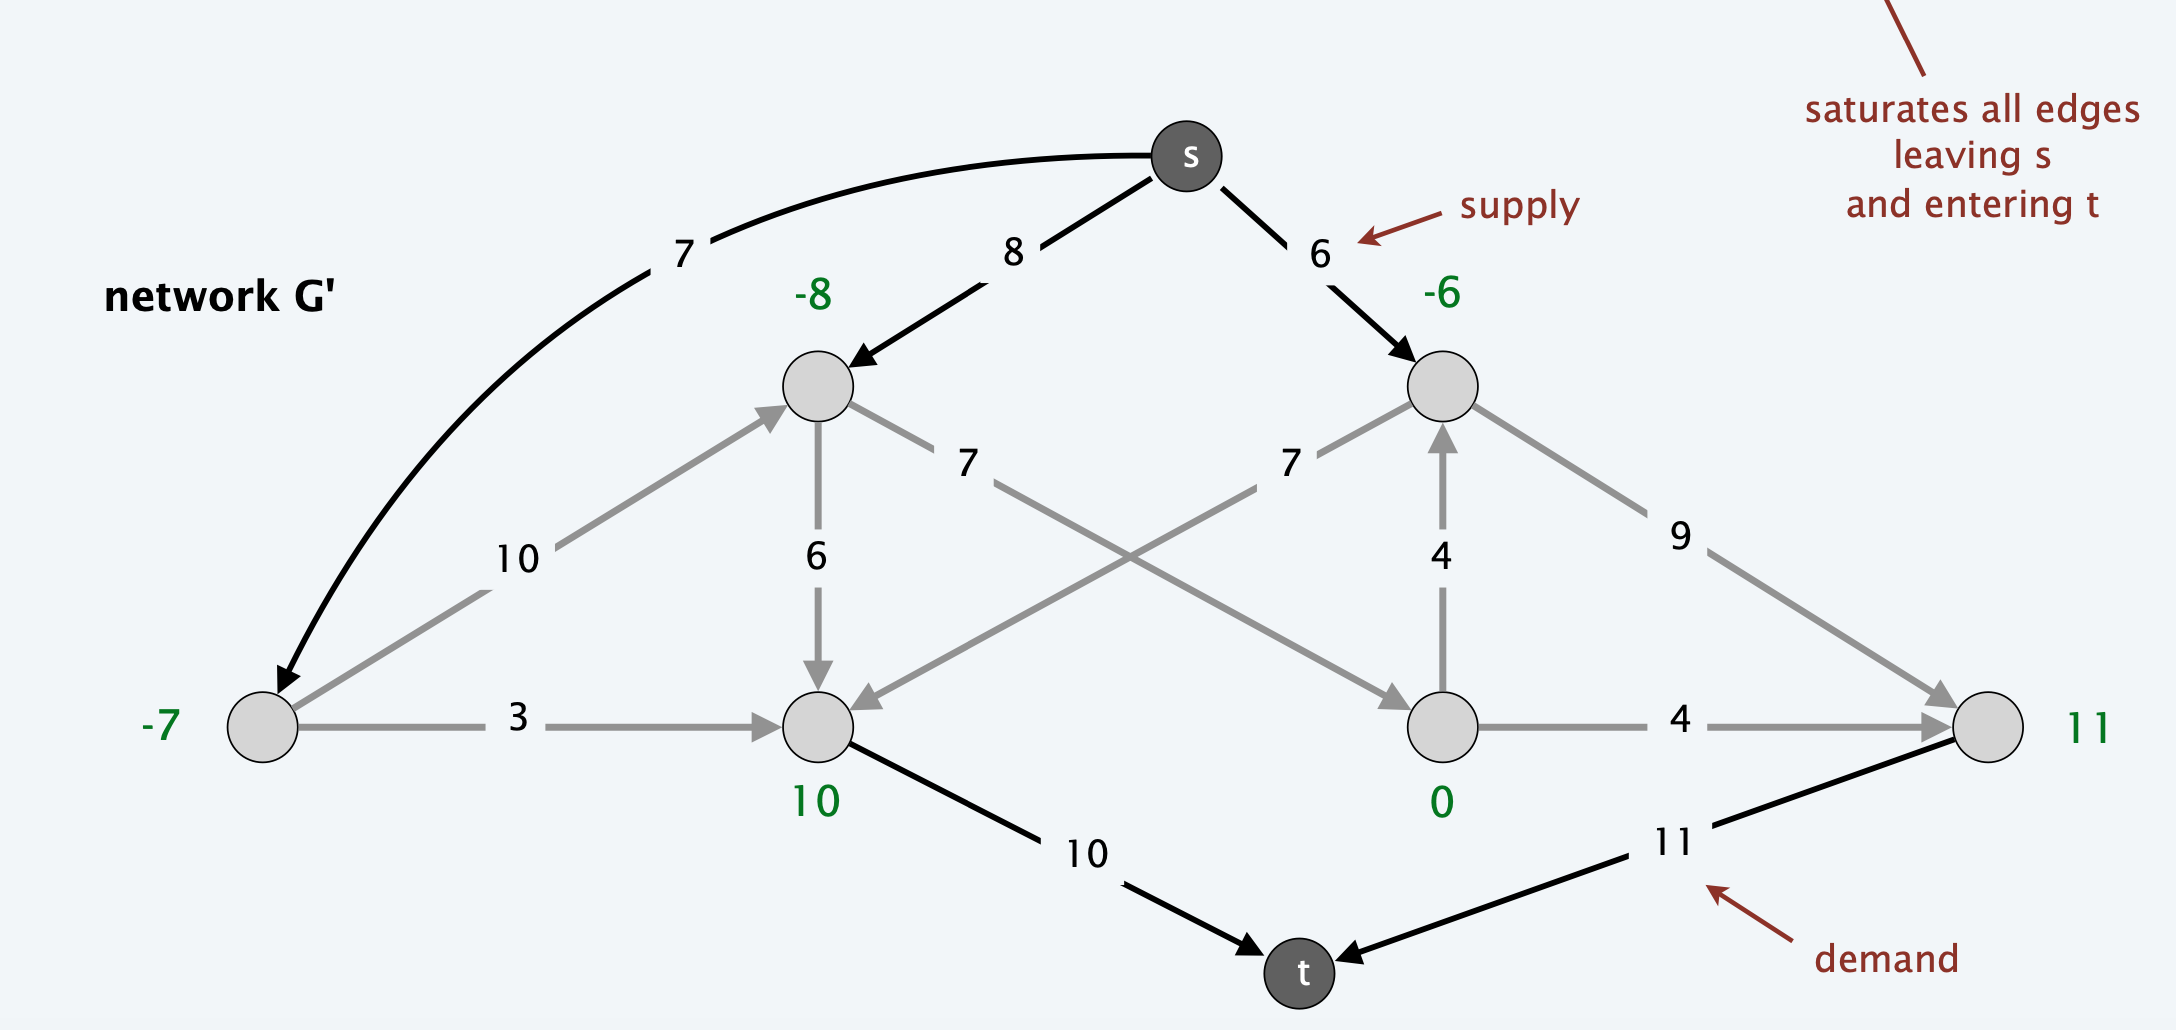
\includegraphics[width=0.6\textwidth ]{maxFlowCirculation}
    \caption{Instance of the Circulation problem with source and sink}
\end{figure}

\begin{claim}
    Given (V, E, c, d), there does not exist a circulation iff there exists a node partition (A, B) such that $\sum _{v \in B} d(v) > cap(A, B).$
\end{claim}\\

\begin{proof}
    By construction, simply looking at the minimum cut of G'.
\end{proof}\\

\emph{Circulation with Lowerbound:}\\\\
Same as before, the problem is the following: Given (V, E, l, c, d), (with l(e) that express lowerbound on $\forall e \in E$) does exist a feasible circulation?\\
The solution is the same as before, modeling the lowerbound problem as a circulation with demands:

\begin{figure}[H]
    \centering
    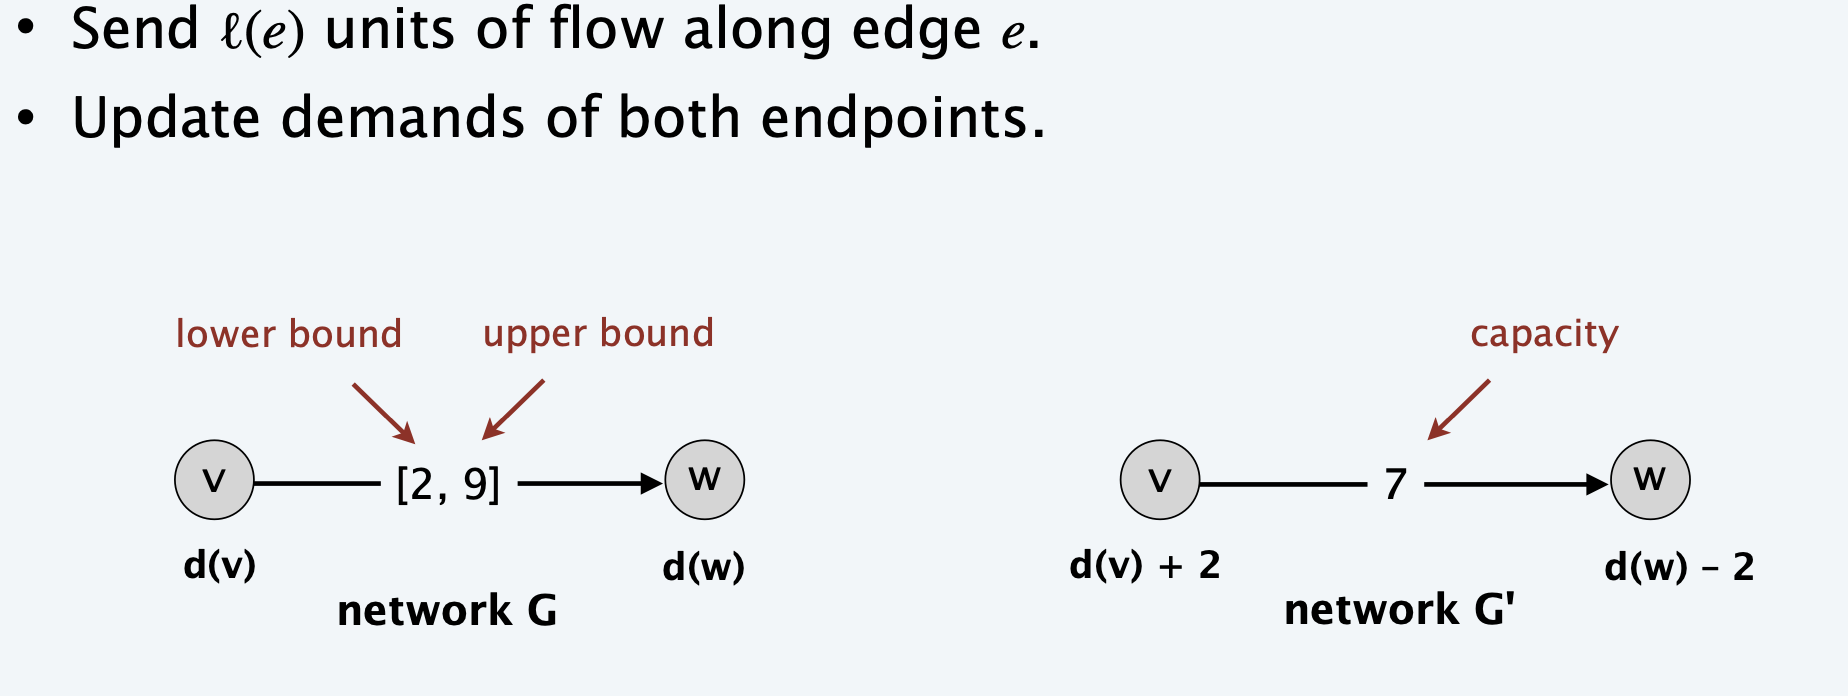
\includegraphics[width=0.6\textwidth ]{lowerbound}
    \caption{Instance of the Circulation problem with lowerbound}
\end{figure}

\begin{claim}
    There exists a circulation in G iff there exists a circulation in G'. Moreover, if all demands, capacities, and lower bounds in G are integers, then there is a circulation in G that is integer-valued.
\end{claim}\\

\begin{proof}
    By construction: f(e) is a circulation in G iff f '(e) = f (e) – l(e) is a circulation in G'.
\end{proof}\\

\subsection{Survey Design}

Design survey asking n consumers about n products but you can only survey consumer i about product j if they own it, you can ask consumer i between ci and ci' questions and only between pj and pj' consumers about product j, the goal is to design a survey that meets these specs, if possible.\\

\emph{Solution}: Model as circulation problem with lower bounds:add edge (i, j) if consumer j owns product i, connect every product to t and every client to s and lastly connect t to s: the integrality circulation is a feasible survey design.

\begin{figure}[H]
    \centering
    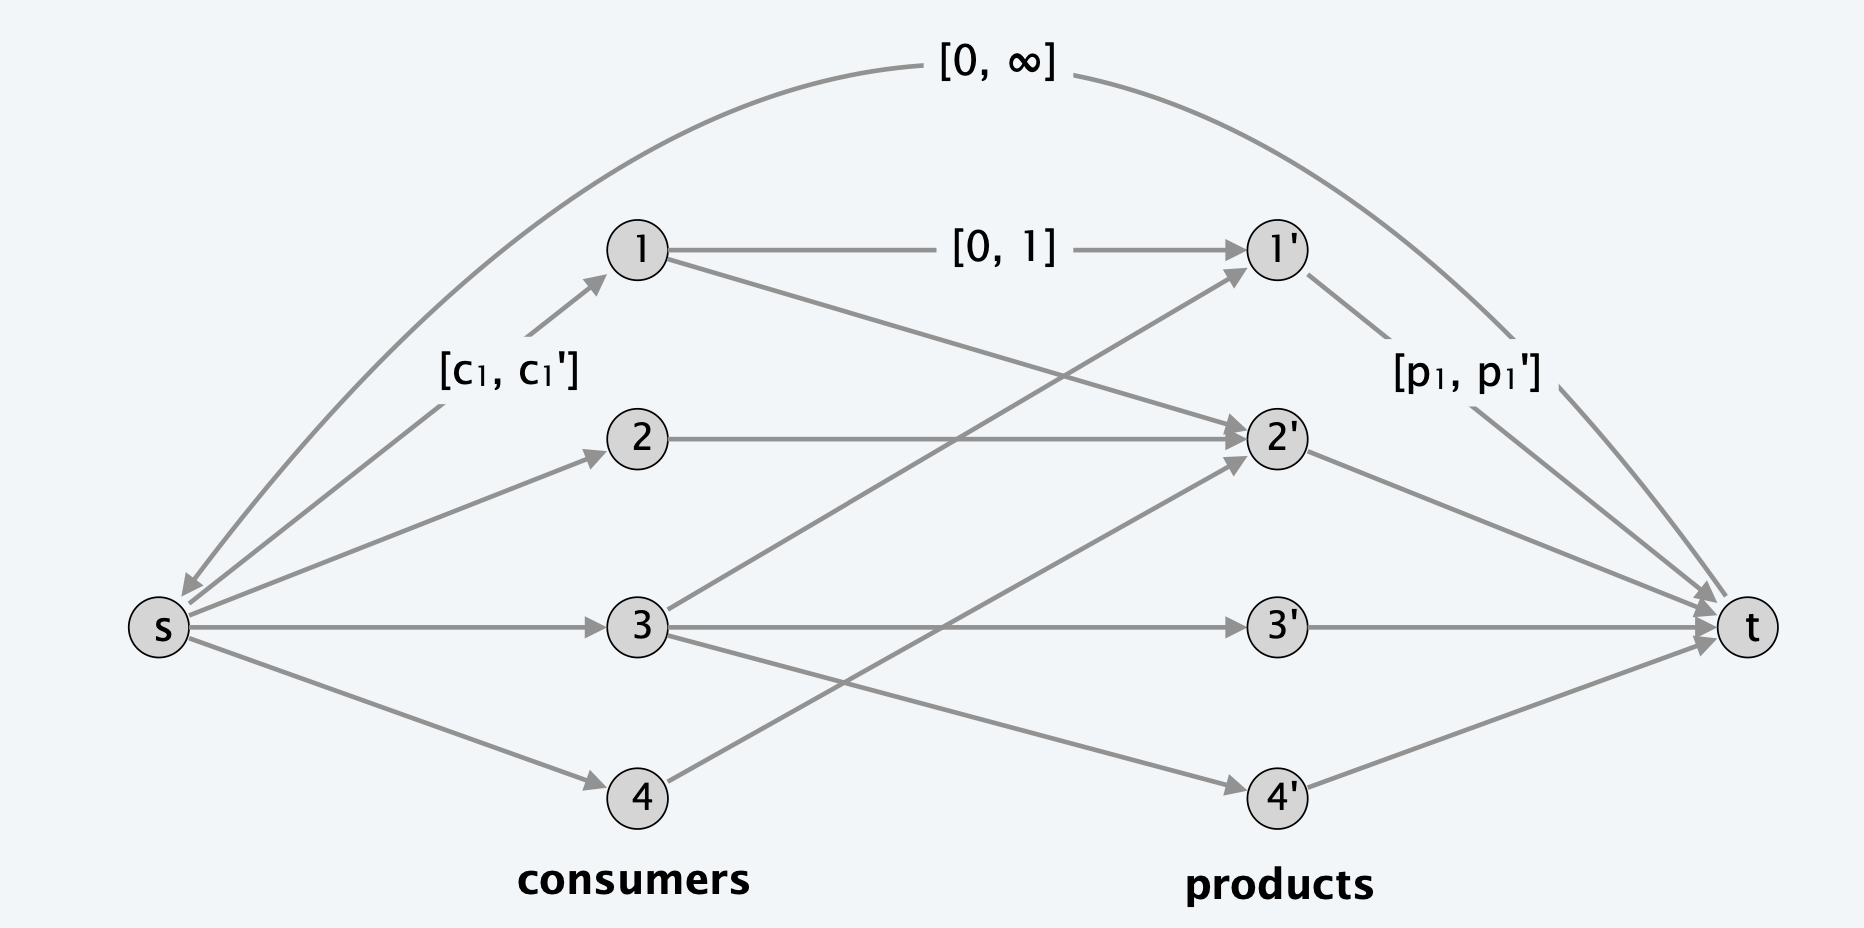
\includegraphics[width=0.6\textwidth ]{survey}
    \caption{Instance of the Survey Problem}
\end{figure}

\subsection{Airline Scheduling}

Airline Scheduling is Complex computational problem faced by nation's airline carriers. Produces schedules that are efficient in terms of: equipment usage, crew allocation, customer satisfaction
and in presence of unpredictable issues like weather, breakdowns.\\
The solution proposed below is a "toy problem" because we can: reusing flight multiple times, each
flight i leaves origin $o_{i}$ at time si and arrives at destination di destination at time $f_{i}$.The goal is to minimize number of flight crews.

\begin{figure}[H]
    \centering
    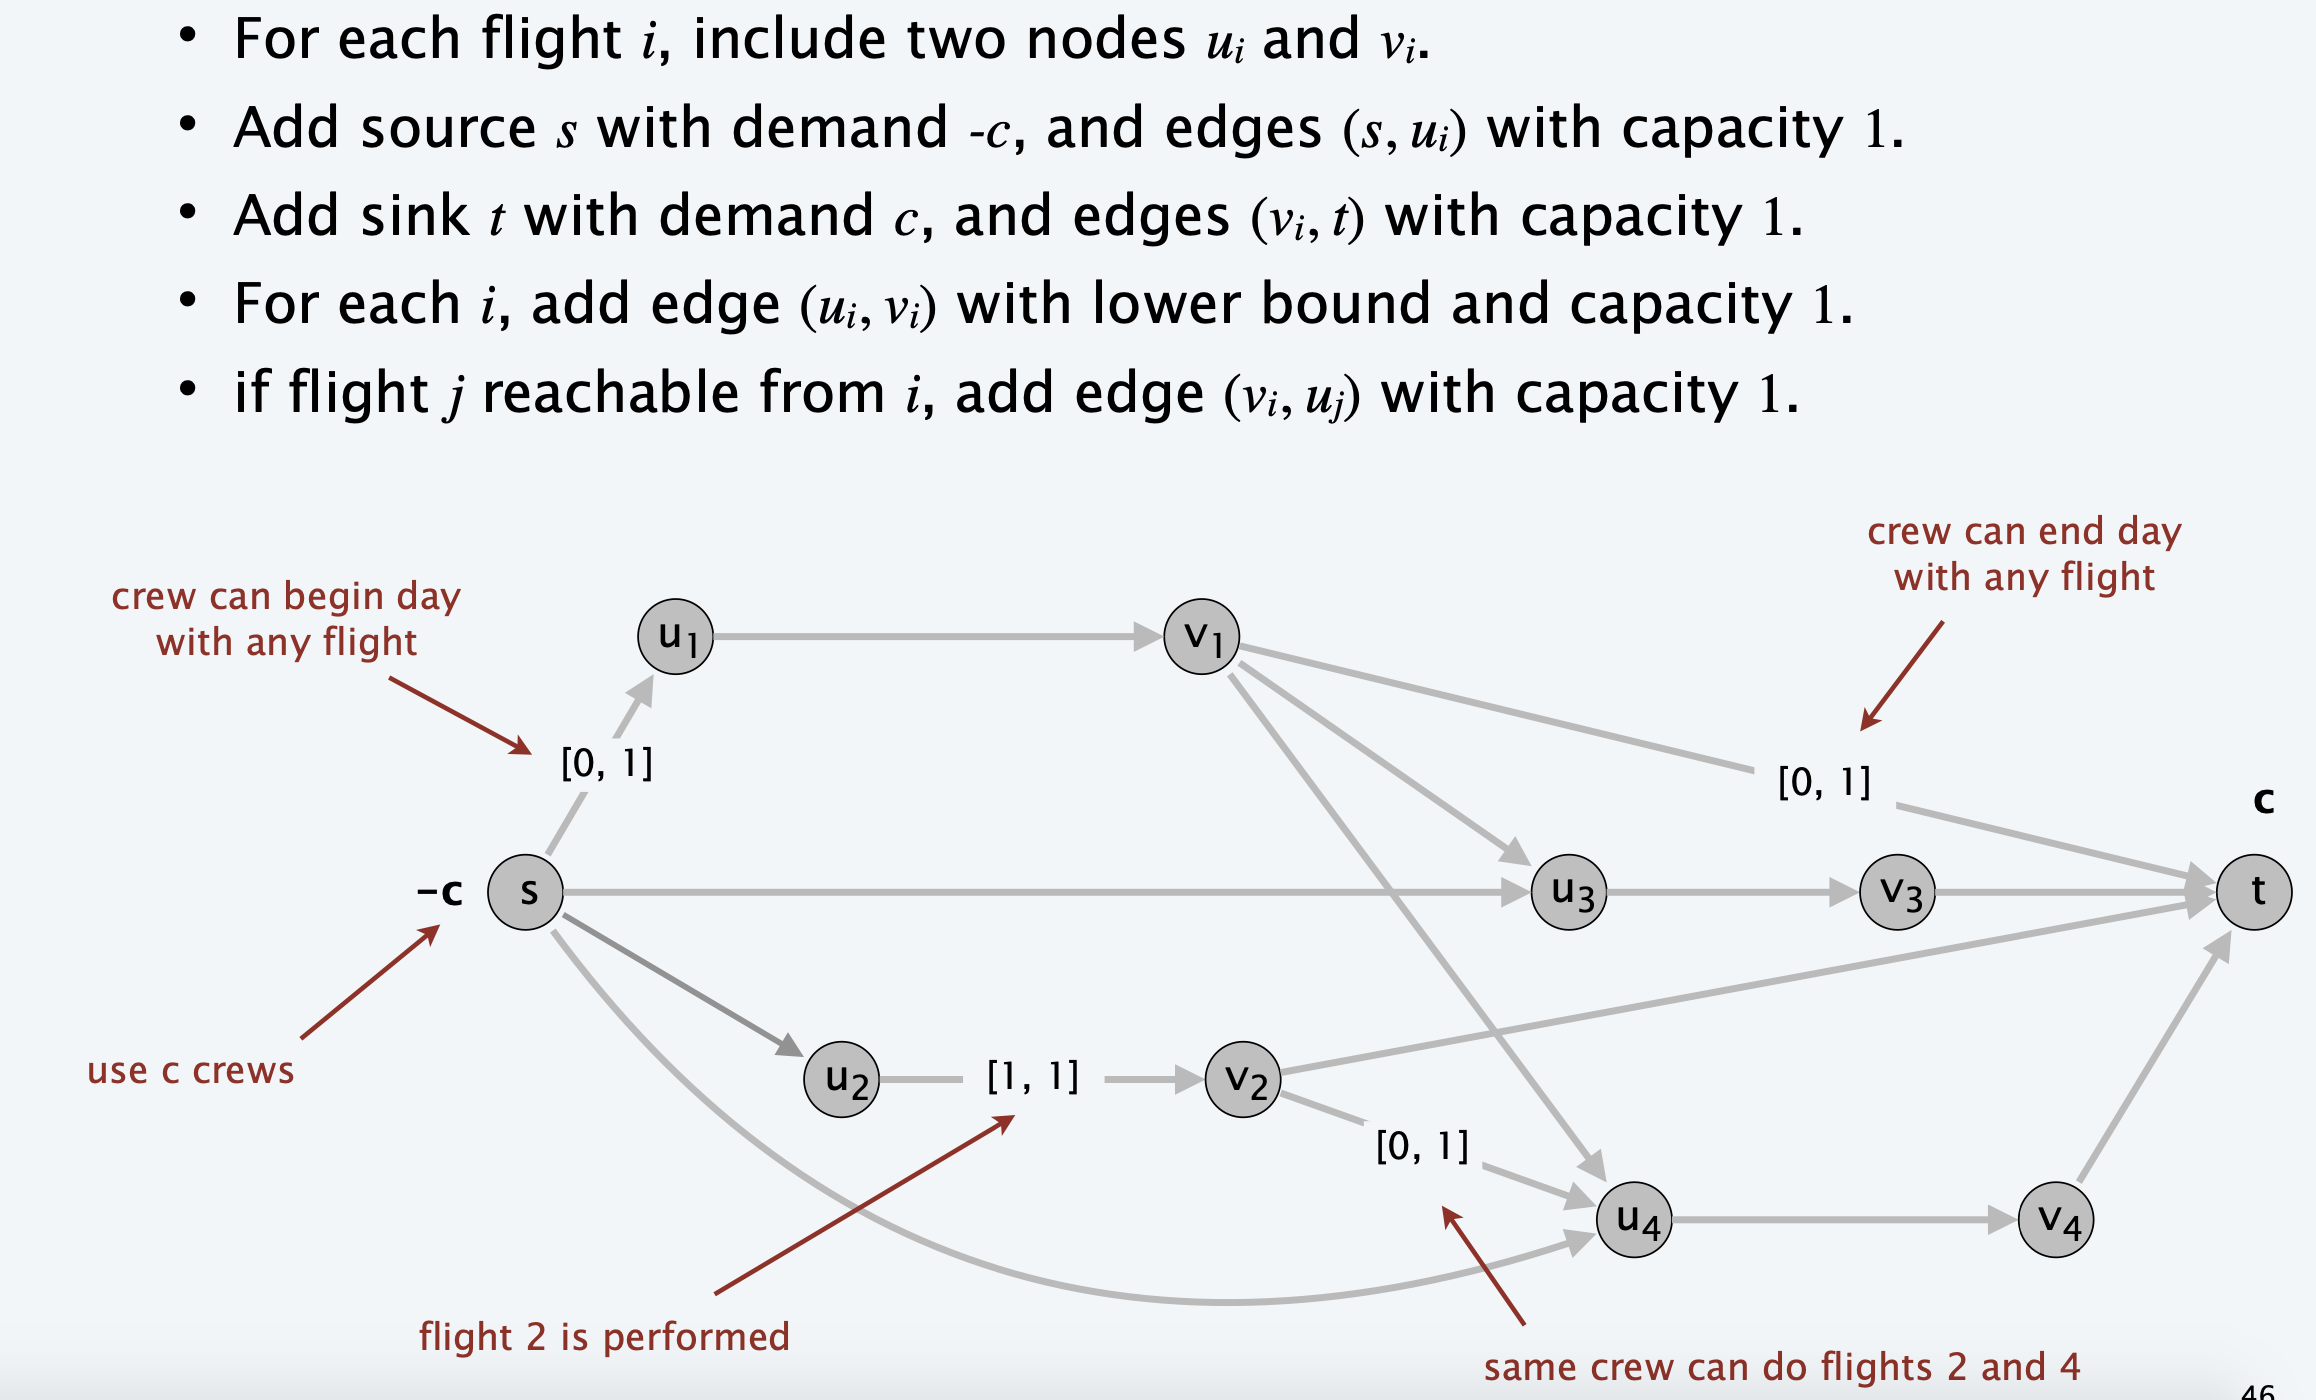
\includegraphics[width=0.6\textwidth ]{airline}
    \caption{Instance of the Airline Problem}
\end{figure}

\begin{claim}
    The airline scheduling problem can be solved in $O(k^{3} log k)$ time, with k = number of flights.
\end{claim}

\begin{proof}
    The number c (of crews is unknown) we have $O(k)$ nodes and $O(k^{2})$ edges so, at most, k crews are needed and by solving the k-circulation problem with at most, k augmenting paths, we obtain $O(k^{3} log k)$ .
\end{proof}

\subsection{Project Selection}
Having a set of possible projects P : project v has associated revenue $p_{v}$, a set of prerequisites E : if $(v, w) \in E$, cannot do project v unless also do project w. A subset of projects $A \subseteq P$ is feasible if the prerequisite of every project in A also belongs to A. Given a set of projects P and prerequisites E, choose a feasible subset of projects to maximize revenue.

\begin{figure}[H]
    \centering
    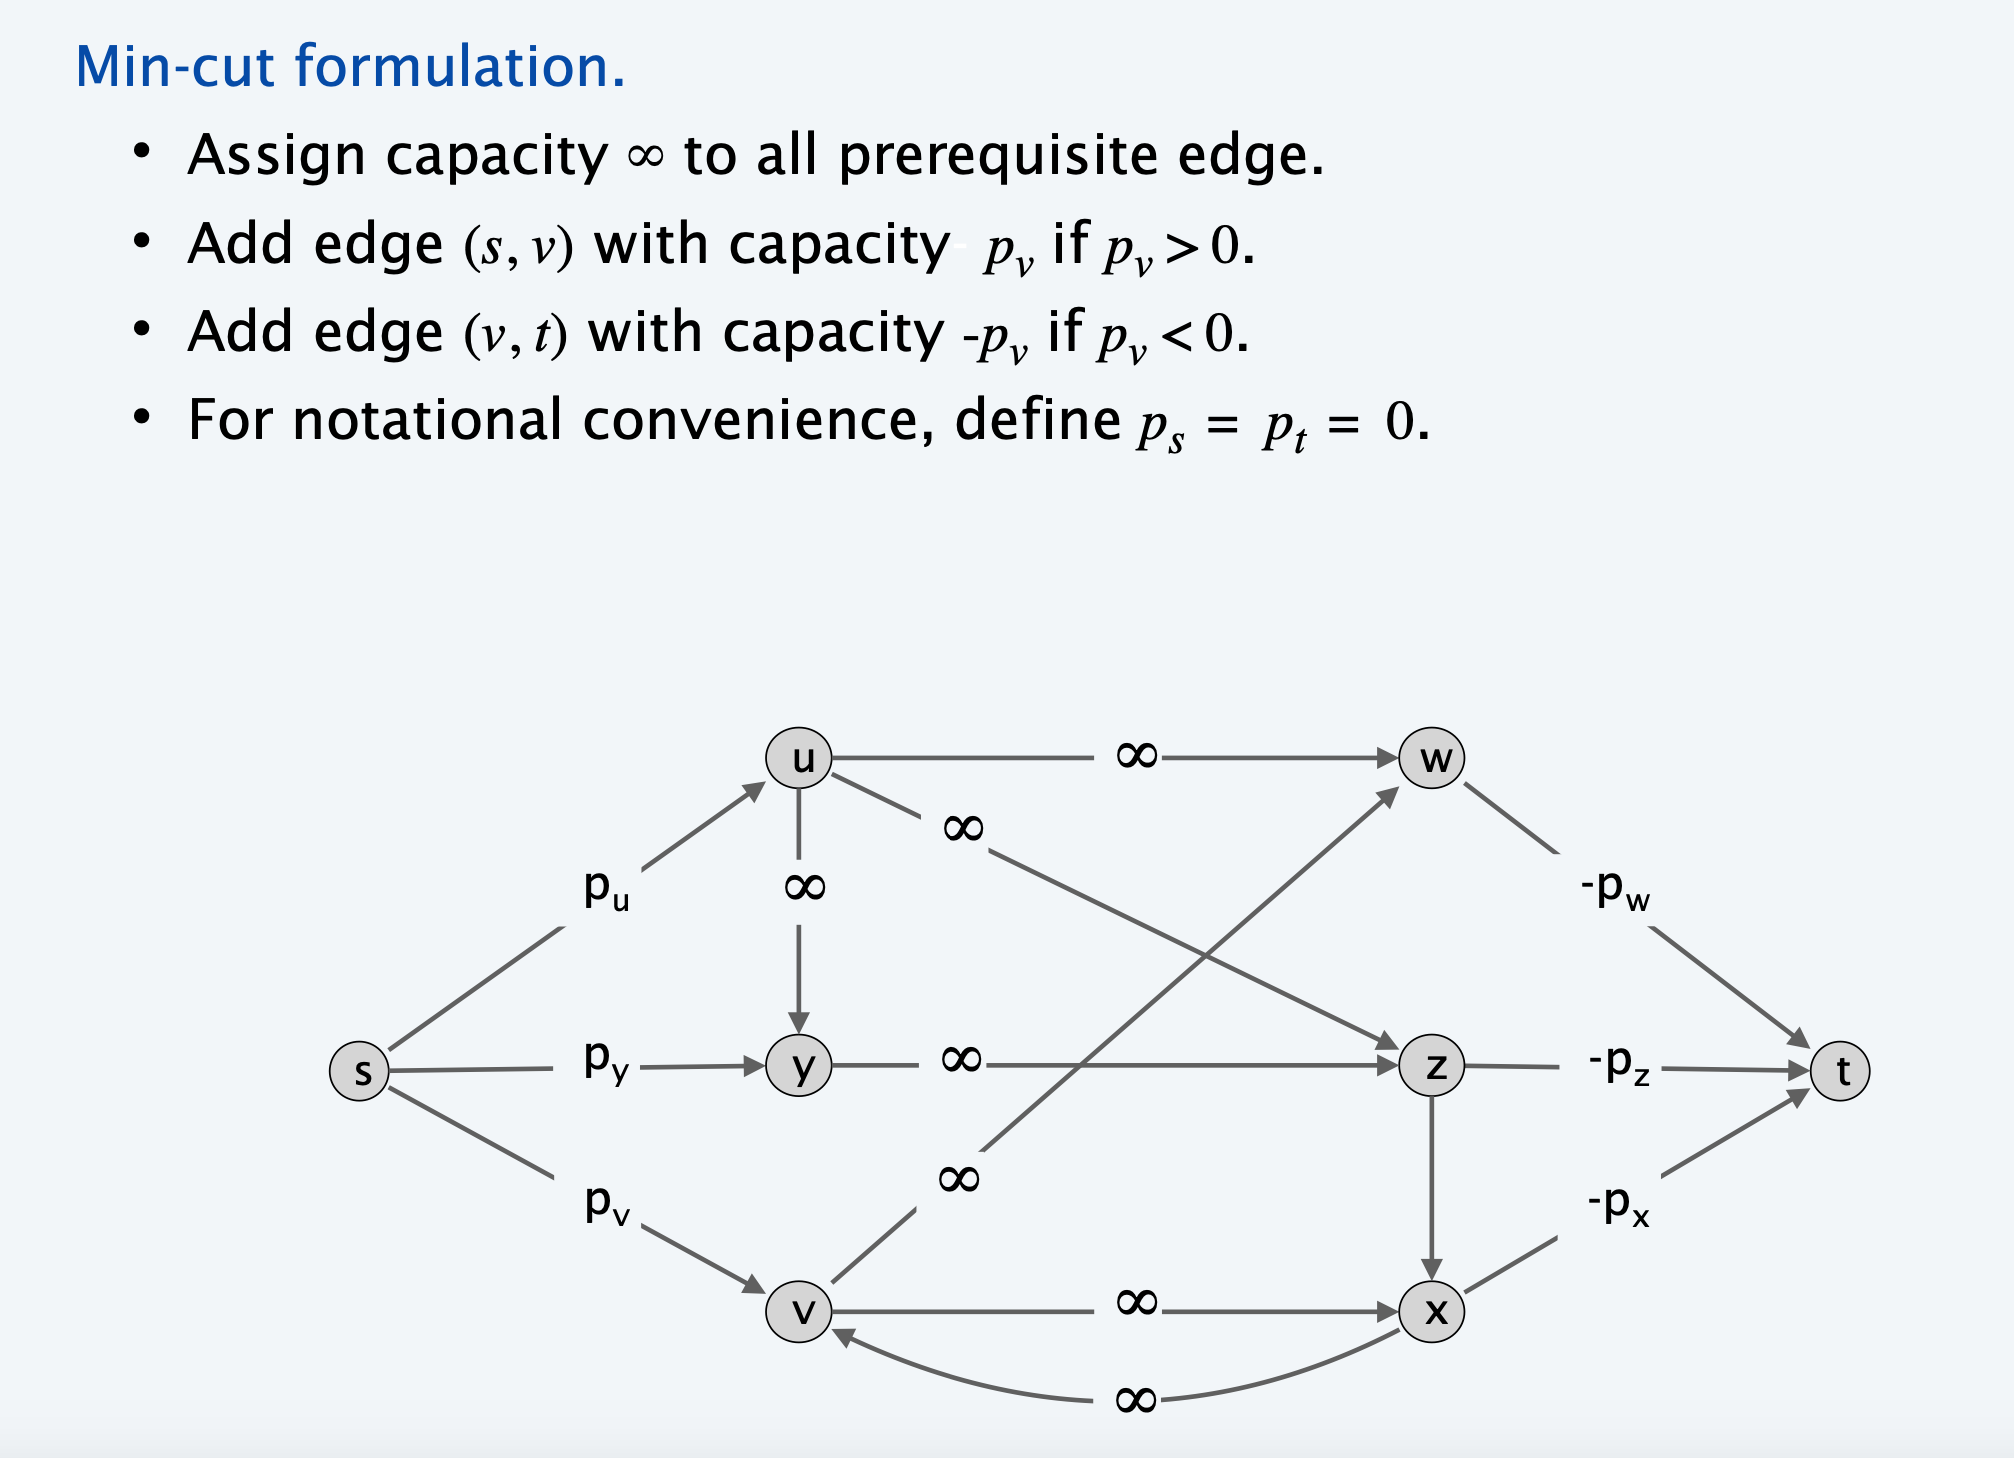
\includegraphics[width=0.6\textwidth ]{projects}
    \caption{Instance of the Projects selection Problem}
\end{figure}

\begin{claim}
    (A, B) is min cut iff A − $\{ s \}$ is optimal set of projects.
\end{claim}\\

\begin{proof}
    Infinite capacity edges ensure $A − \{ s \}$ is feasible.
\end{proof}

\subsection{Baseball Game}
Which teams have a chance of finishing the season with the most wins? Ex:  Montreal is mathematically eliminated (Montreal finishes with $\leq$ 80 wins but Atlanta has already 83). The answer depends not only on how many games already won and left to play, but on whom they're against.\\So we have a set of teams S, distinguished team $z \in S$, team x has won $w_{x}$ games already and x and y play each other $r_{xy}$ additional times.\\\\
Given the current standings, is there any outcome of the remaining games in which team z finishes with the most (or tied for the most) wins?

\begin{figure}[H]
    \centering
    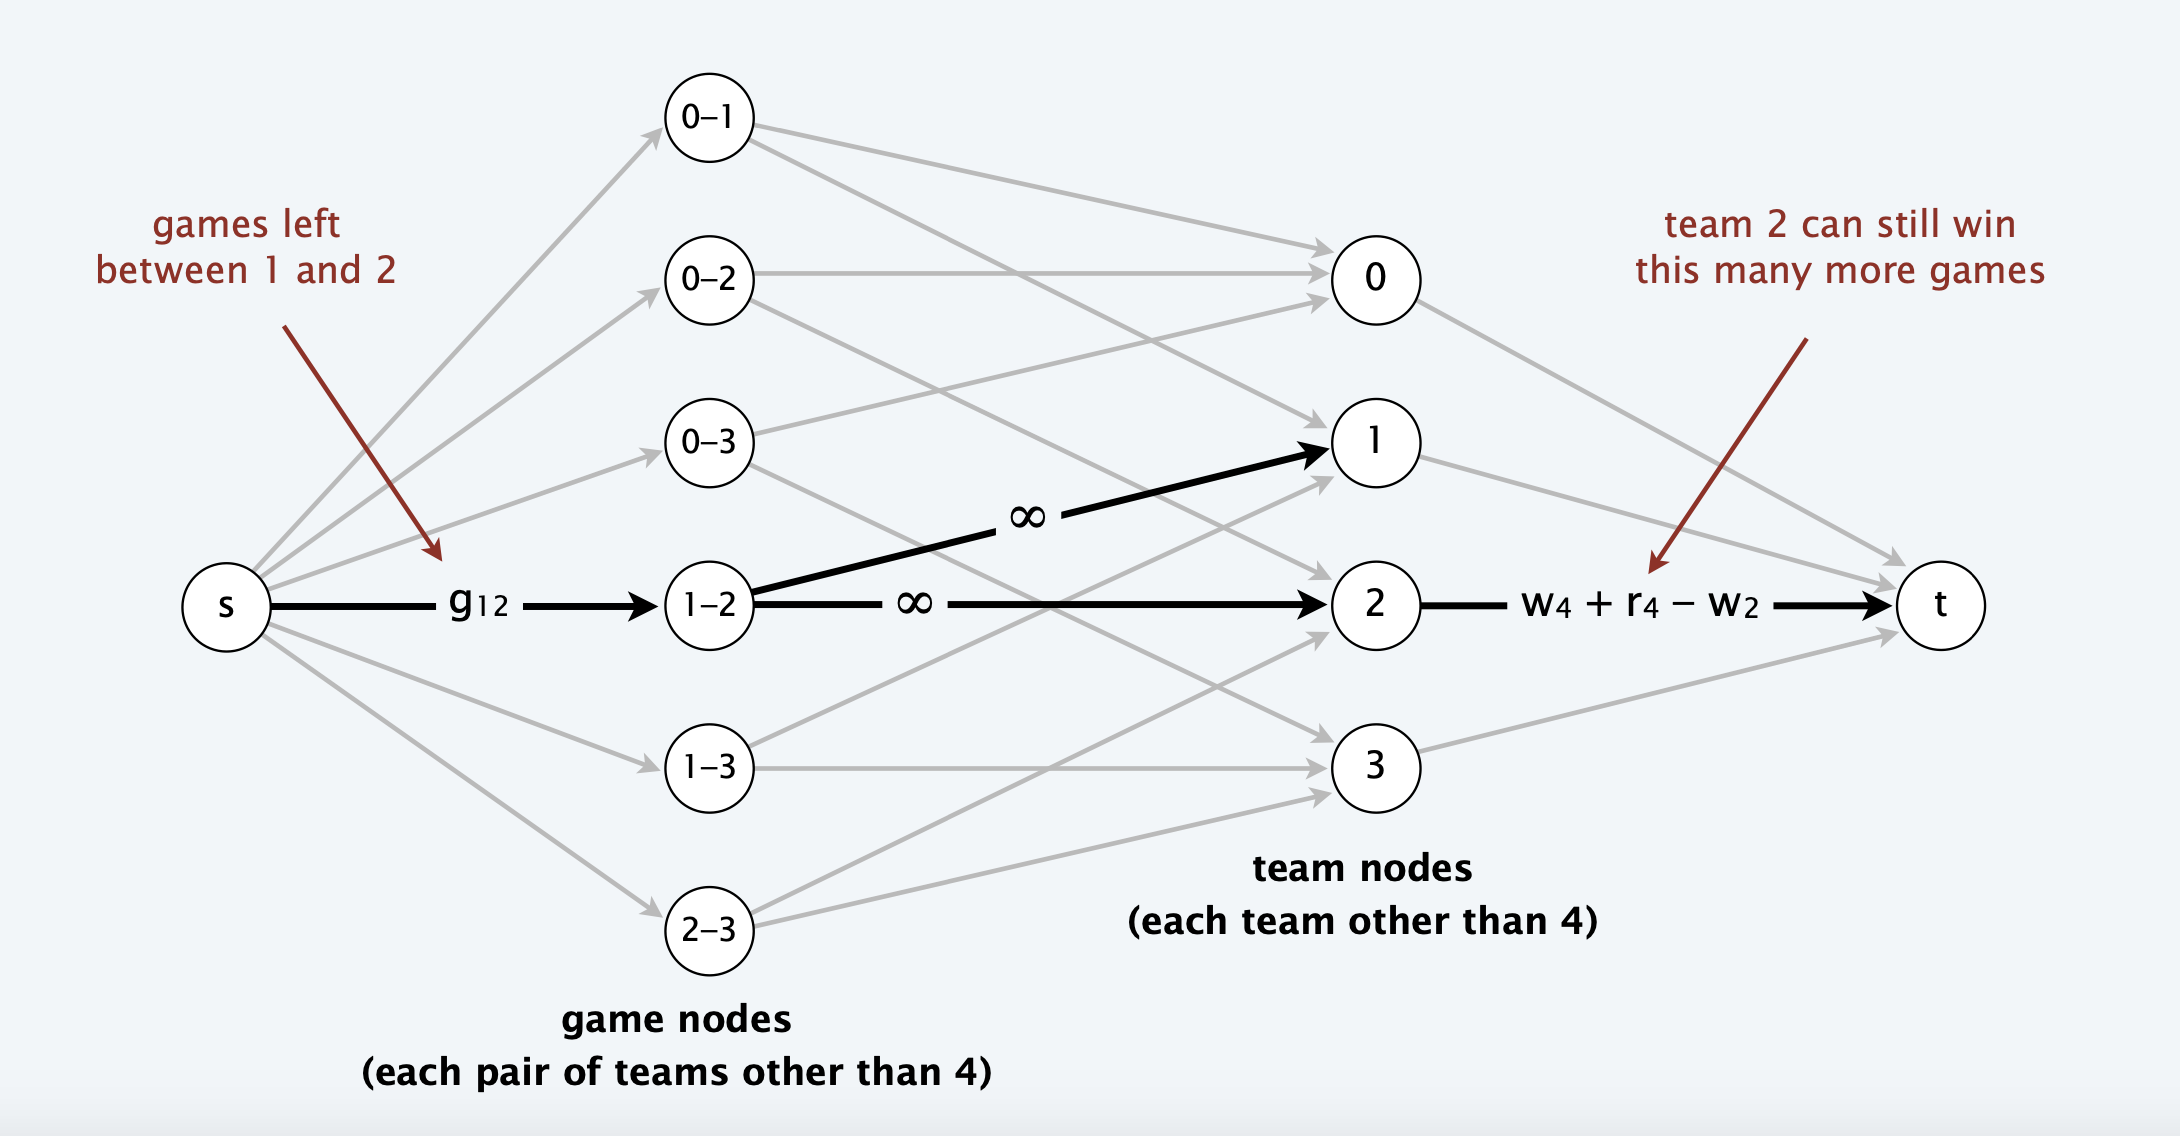
\includegraphics[width=0.6\textwidth ]{baseballFlow}
    \caption{Instance of the Baseball Game Problem}
\end{figure}

\begin{claim}
    Team 4 not eliminated iff max flow saturates all edges leaving s.
\end{claim}\\

\begin{proof}
    Integrality theorem $\Rightarrow $ each remaining game between x and y added to number of wins for team x or team y, the capacity on (x, t) edges ensure no team wins too many games.
\end{proof}

\begin{figure}[H]
    \centering
    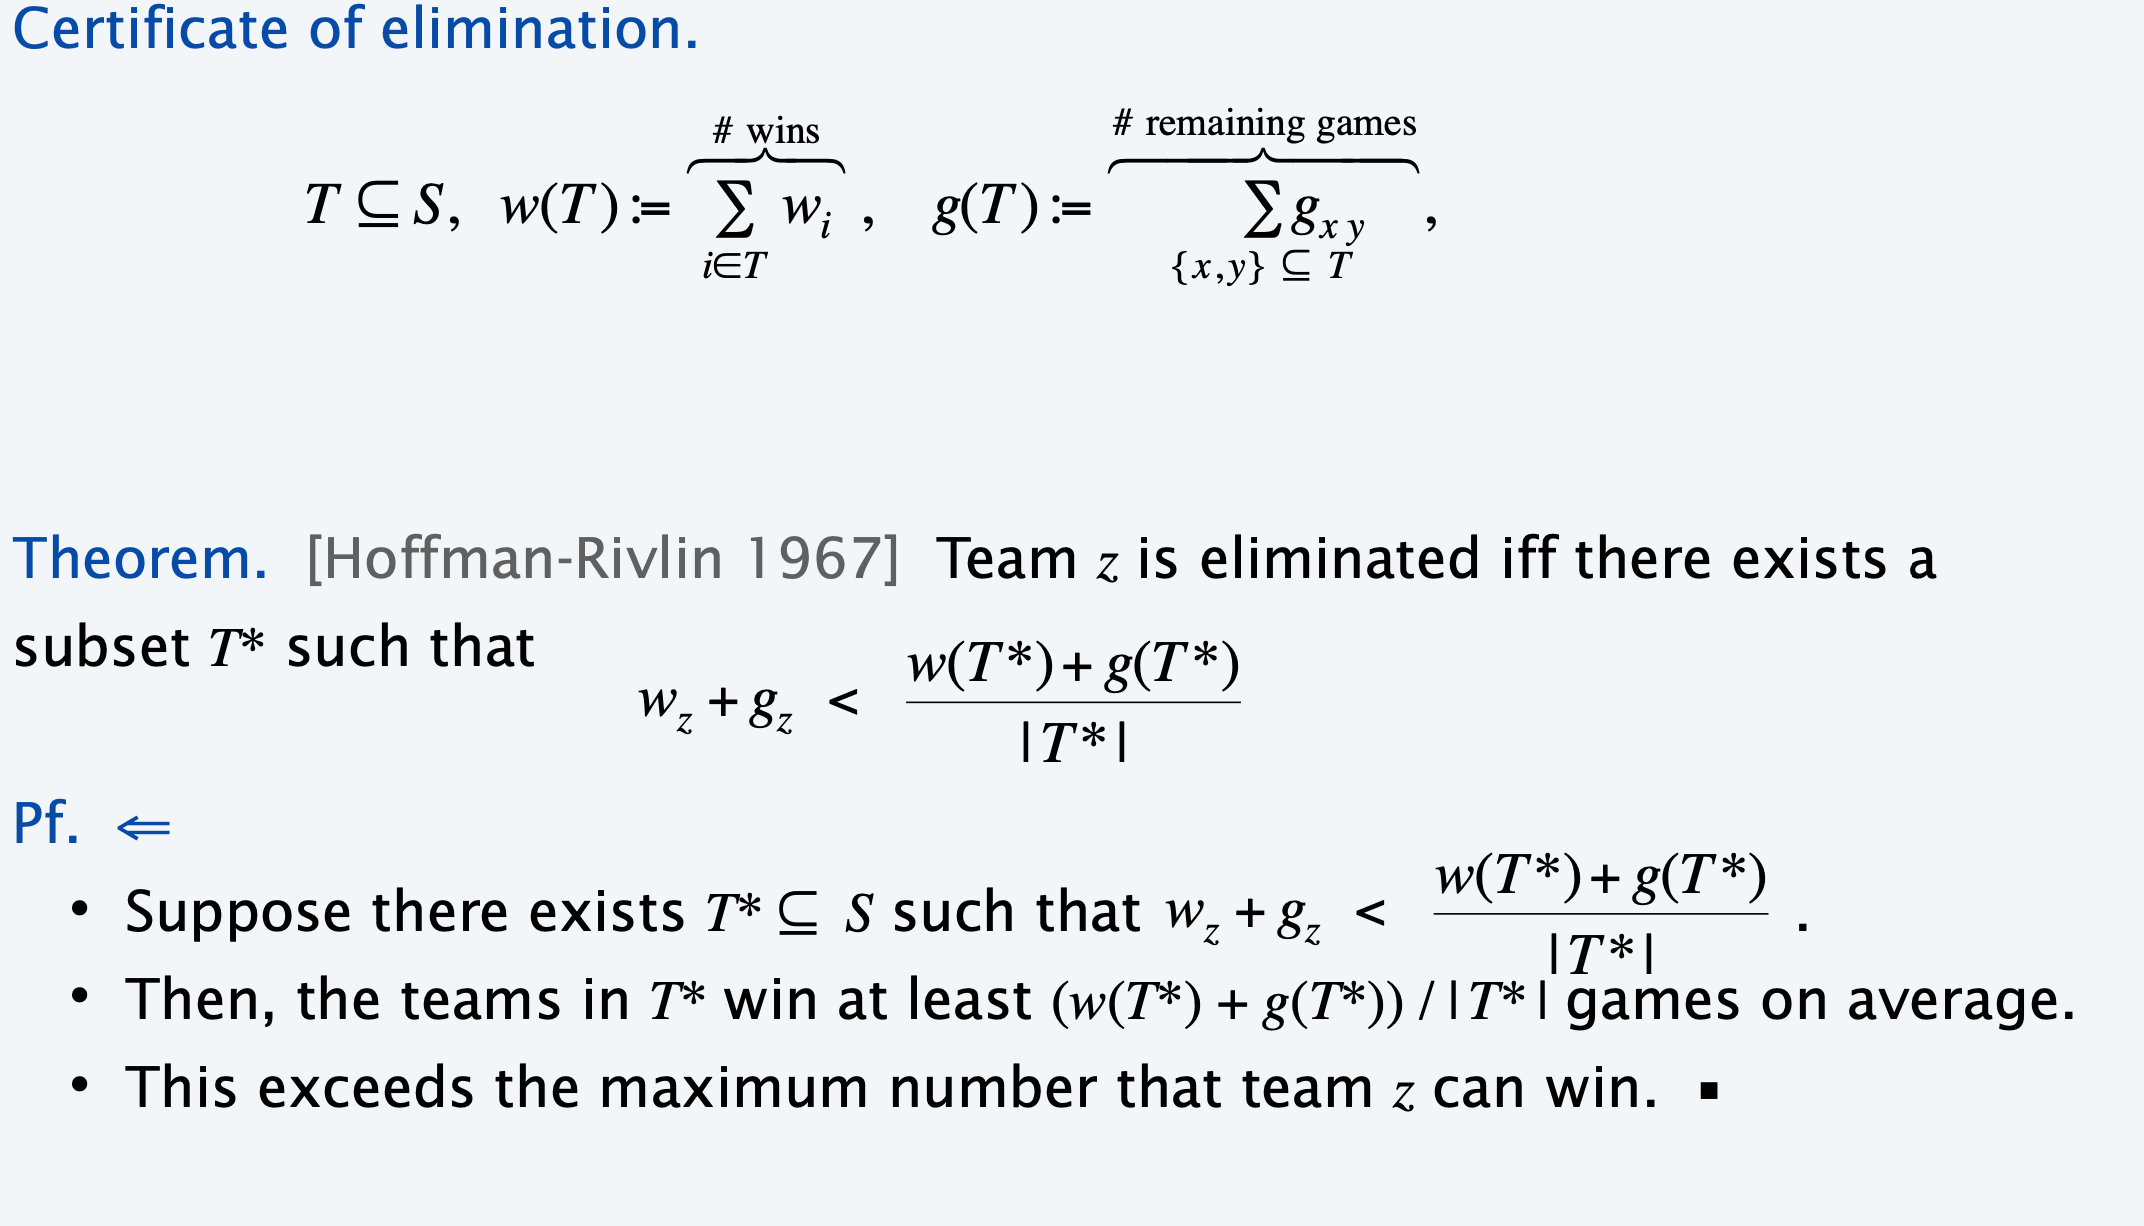
\includegraphics[width=0.6\textwidth ]{baseballElimination}
\end{figure}

\clearpage

